\documentclass[12pt]{amsart}
%\pagestyle{empty} 
\setlength{\topmargin}{-0.3in} % usually -0.25in
\addtolength{\textheight}{.75in} % usually 1.25in
\addtolength{\oddsidemargin}{-1.0in}
\addtolength{\evensidemargin}{-1.0in}
\addtolength{\textwidth}{2.0in} %\setlength{\parindent}{0pt}

% macros
\usepackage{wrapfig,caption,palatino}
\usepackage{amssymb,xspace}
\usepackage[final]{graphicx}
\usepackage[colorlinks=true]{hyperref}

\newcommand{\regfigure}[3]{\includegraphics[height=#2in,width=#3in]{#1.eps}}

\newtheorem*{lem*}{Lemma}

\newcommand{\mtt}{\texttt}
\newcommand{\mtl}[1]{{\texttt{>>#1}}}
\usepackage{alltt}
\usepackage{verbatim} % for "comment" environment
\newcommand{\mfile}[1]
{\medskip\begin{quote} \begin{alltt}\input{C:/MATLABR11/work/#1.m}\end{alltt} \end{quote}\medskip}

\newcommand{\CC}{{\mathbb{C}}}
\newcommand{\RR}{{\mathbb{R}}}
\newcommand{\eps}{\epsilon}
\newcommand{\ZZ}{{\mathbb{Z}}}
\newcommand{\ZZn}{{\mathbb{Z}}_n}
\newcommand{\NN}{{\mathbb{N}}}
\newcommand{\bu}{\mathbf{u}}
\newcommand{\bv}{\mathbf{v}}
\newcommand{\ip}[2]{\mathrm{\left<#1,#2\right>}}
\newcommand{\erf}{\operatorname{erf}}
\newcommand{\spn}{\operatorname{span}}

\newcommand{\Matlab}{\textsc{Matlab}\xspace}
\newcommand{\Octave}{\textsc{Octave}\xspace}
\newcommand{\pylab}{\textsc{pylab}\xspace}
\newcommand{\MOP}{\textsc{Matlab}\big|\textsc{Octave}\big|\textsc{pylab}\xspace}

\newcommand{\prob}[1]{\bigskip\bigskip\noindent\large\textbf{#1.} \normalsize}
\newcommand{\bookprob}[1]{\bigskip\bigskip\noindent\large\textbf{Exercise #1.} \normalsize}
\newcommand{\ppart}[1]{\medskip\noindent\large\textbf{\emph{#1})}\normalsize}

\newcommand{\textbook}{\textsc{Trefethen \& Bau}}

\begin{document}

\begin{center}
\Huge Math 661 Optimization
\end{center}

\thispagestyle{empty}

Mathematical optimization is essential technology for science, engineering, and economics.  This course, a graduate-level introduction to continuous optimization, focusses on ideas, algorithms, and applications.  Mathematical rigor, proof, is used when appropriate.

Course Website: \url{https://bueler.github.io/opt/}

\begin{wrapfigure}{r}{0.5\textwidth}
  \centering
    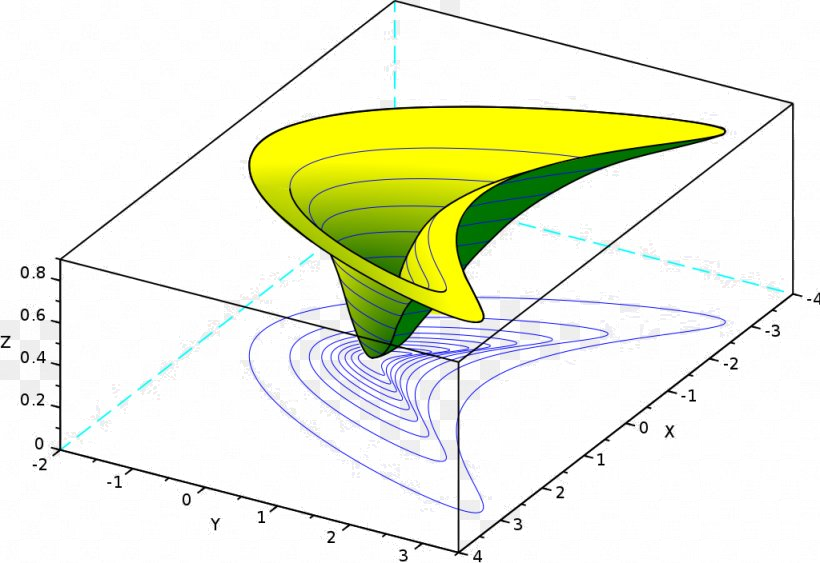
\includegraphics[width=0.5\textwidth]{../images/banana.png}
\captionsetup{margin=1.2cm}
  \caption{Birds}
\end{wrapfigure}

Topics:

\begin{itemize}
\item    Continuous optimization, both nonlinear and linear.
\item     Simplex method for linear programming. ("Linear programming" refers to optimization of a linear function subject to linear constraints.)
\item     Iterative methods for unconstrained problems, including Newton and quasi-Newton methods.
\item     Line search and trust region methods.
\item     Constrained problems and Karush-Kuhn-Tucker conditions.
\item     Linear algebra related to the above topics.
\item     Convergence theorems for some methods.
\item     Practical work with the computer. Examples from applications.
\end{itemize}


\begin{wrapfigure}{l}{0.25\textwidth}
  \centering
    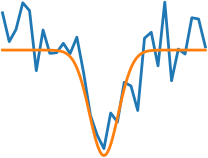
\includegraphics[width=0.25\textwidth]{../images/smooth-noisy.png}
\captionsetup{margin=1.2cm}
  \caption{Birds}
\end{wrapfigure}

Goals and Outcomes:
The goal of this applied mathematics course is to be able to understand optimization problems as they arise in applied contexts, select algorithms, and apply optimization software based on understanding of theory and standard examples. Understanding of concepts should suffice for the student to assess claims about optimization software performance. Increased student competence with general scientific computing is also a goal.

Textbook:
Griva, Nash, and Sofer, Linear and Nonlinear Optimization, 2nd ed., SIAM Press 2009 

\begin{wrapfigure}{r}{0.5\textwidth}
  \centering
    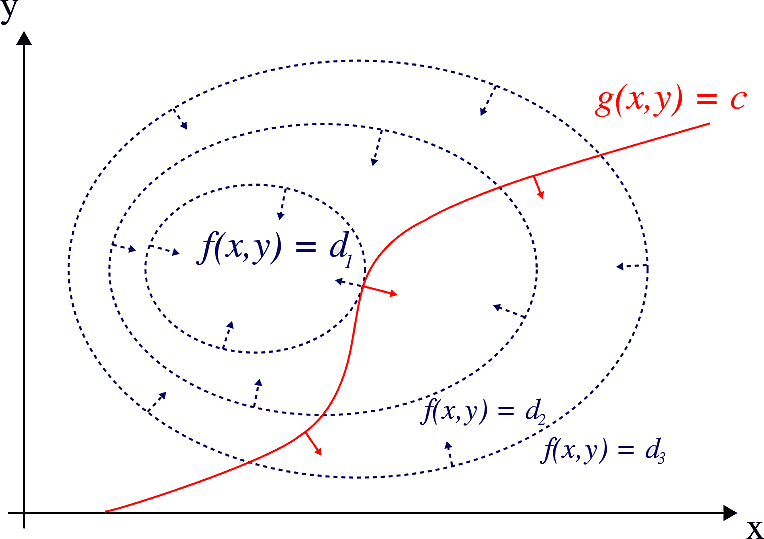
\includegraphics[width=0.5\textwidth]{../images/lagrange.png}
\captionsetup{margin=1.2cm}
  \caption{Birds}
\end{wrapfigure}

Prerequisites: 
\end{document}

